\documentclass[a4paper,14pt]{extarticle} % the default article class is limited to 12pt, but you can go up to 14, 17 or 20 points if you use the extarticle class:
\usepackage{cmap} % make LaTeX PDF output copy-and-pasteable
\usepackage[T2A]{fontenc}
\usepackage[utf8]{inputenc}
\usepackage[english,ukrainian]{babel}

\usepackage{amssymb,amsfonts,mathtools,amsmath,cite,enumerate,float}
\usepackage{indentfirst} % set an additional space before a paragraph at the begining of new section
\usepackage{setspace}
\usepackage{textcomp}

\usepackage{import} % for adding a file by path https://tex.stackexchange.com/questions/246/when-should-i-use-input-vs-include

\usepackage{geometry} 
\geometry{left=1.25cm}
\geometry{right=1.25cm}
\geometry{top=1cm}
\geometry{bottom=2cm}

\usepackage[table,xcdraw,dvipsnames]{xcolor}
\usepackage{color}
% 1) tutorial about xcolor:  https://www.overleaf.com/learn/latex/Using_colours_in_LaTeX
% 2) huge tutorial about xcolor: https://latex-tutorial.com/color-latex/ 
% 3) RGB calculator: https://www.w3schools.com/colors/colors_rgb.asp

\usepackage{hyperref}
\definecolor{linkcolor}{HTML}{0000FF}
\definecolor{urlcolor}{HTML}{0000FF} 
\hypersetup{pdfstartview=FitH, linkcolor=linkcolor, urlcolor=urlcolor, colorlinks=true}

\usepackage{graphicx}
\usepackage{wrapfig}
\graphicspath{{Screenshots/}} % path to images

\parskip=1mm %space between paragraphs

\usepackage{listingsutf8} % for code (origin: \usepackage{listings})

\lstset{
    frame=single, %lines
    language=Python,
    aboveskip=3mm,
    belowskip=3mm,
    columns=flexible,
    basicstyle={\small\ttfamily},
    numbers=left,
    numberstyle=\tiny\color{gray},
    commentstyle=\color{OliveGreen},
    stringstyle=\color{Mahogany},
    morestring=[b]''',
    showstringspaces=false,
    keywordstyle=\bfseries\color{blue},
    emph={[1]import, as, for, return}, emphstyle={[1]\bfseries\color{magenta}},
    emph={[2]range}, emphstyle={[2]\bfseries\color{brown}},
    breaklines=true,
    breakatwhitespace=true,
    tabsize=4,
    extendedchars=false, % to use ukrainian text in a code
    inputencoding=utf8 % to use ukrainian text in a code
}

\begin{document}

\import{Title/}{title}

\newpage

\section*{Мета}

Ознайомитись з використанням AWS DynamoDB (serverless database).

\section*{Завдання} 

\begin{itemize}
    \item Спроектувати структуру даних (таблицю);
    \item Вивчити способи роботи з даними засобами DynamoDB;
    \item Виконати завдання відповідно до варіанту (GUI, засобами AWS CLI, NoSQL Workbench та Python -- останнє за бажанням).
\end{itemize}

\section*{Хід виконання роботи}

\subsection*{1. Робота з таблицею заcобами AWS Management Console}

\subsubsection*{Створення таблиці}

Для створення таблиці засобами AWS Management Console слід увійти в свій акаунт й віднайти розділ <<DynamoDB>> 
самостійно або перейшовши за \href{https://us-east-1.console.aws.amazon.com/dynamodbv2/home?region=us-east-1#dashboard}{посиланням}.

Далі шукаємо у правій частині екрану помаранчеву кнопку <<Create table>>. Після цього вводимо назву таблиці та 
назву стовпця, який буде відігравати роль Primary key для рядків таблиці. Інакше кажучи, слід придумати стовпець, 
елементи якого будуть унікальними для кожного рядка таблиці. 

Наприклад, для структури даних студентів групи роль такого стовпця може відігравати номер залікової книги 
(у кожного студента він свій, а відтак цей номер однозначно характеризуватиме кожного конкретного студента). 
Колонка Primary key може складатися й з двох частин. Наприклад, у випадку тих же студентів можна 
ввести складений ключ: назва групи й порядковий номер студента в групі. Така комбінація теж буде 
унікальною для кожного студента.

У цій лабораторній буде відбуватися робота з даними про курс гривні відносно інших валют. З цими даними ми вже 
працювали у Лабораторній роботі \textnumero2. Таблиця, яку ми намагаємося створити, матиме п'ять колонок:
\begin{align*}
    &\texttt{r030} &&\text{номер запису} \\
    &\texttt{txt} &&\text{назва валюти українською} \\
    &\texttt{rate} &&\text{поточне значення курсу} \\
    &\texttt{cc} &&\text{міжнародний шифр валюти} \\
    &\texttt{exchangedate} &&\text{поточна дата}
\end{align*}

Тож на завершення діалогового вікна створення таблиці крім її імені варто зазначити й  Primary key. У випадку 
структури даних курсу валют я обрав складений Primary key: колонку шифра валют \texttt{cc} й поточної дати 
\texttt{exchangedate} (Рис. \ref{fig:create table AWS MC}).

\begin{figure}[H]
    \center{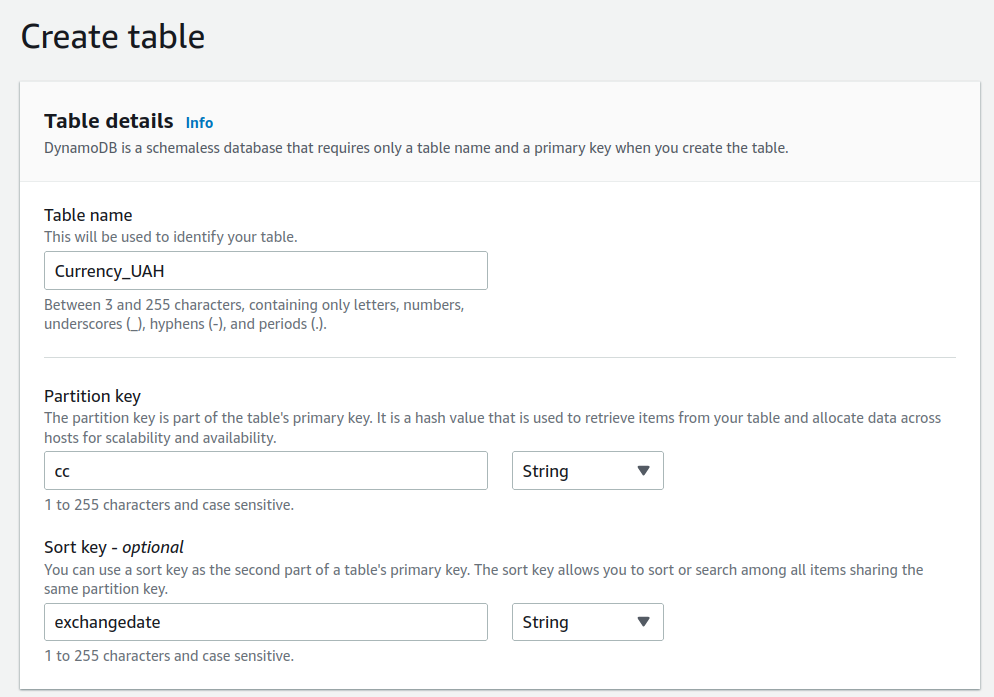
\includegraphics[width=1\linewidth]{1/1.1.png}}
    \caption{Створення таблиці засобами AWS Management Console}
    \label{fig:create table AWS MC}
\end{figure}

\subsubsection*{Додавання рядків до таблиці}

Поступово додамо 5 рядків до новоствореної таблиці <<Currency\_UAH>>. Для цього спершу натиснемо на ім'я таблиці 
в каталозі усіх таблиць DynamoDB. Потім оберемо помаранчеву кнопку <<Explore table items>> 
(Рис.~\ref{fig:explore table items AWS MC}). І наостанок знайдемо <<Create item>>. Введемо значення для вже 
існуючих двох колонок нашого складеного Primary key, а решта інформації додамо інструментом <<Add new attribute>> 
(Рис.~\ref{fig:add an item AWS MC}). Почергово додавши 5 рядків, отримаємо фінальну заповнену структуру даних 
(як це зображено на Рис.~\ref{fig:creation finished AWS MC}).

Отже, алгоритм додавання рядків до новоствореної таблиці виглядатиме так:
\begin{align*}
    &\rightarrow \text{<<Currency\_UAH>>} \\
    &\rightarrow \text{Explore table items} \\
    &\qquad \rightarrow \text{Create item} \\
    &\qquad \rightarrow \text{Fill the data for a Primary key} \\   
    &\qquad \rightarrow \text{Add new attribute} \\
    &\qquad \rightarrow \text{Fill the data for an additional attribute} 
\end{align*}

\begin{figure}[H]
    \center{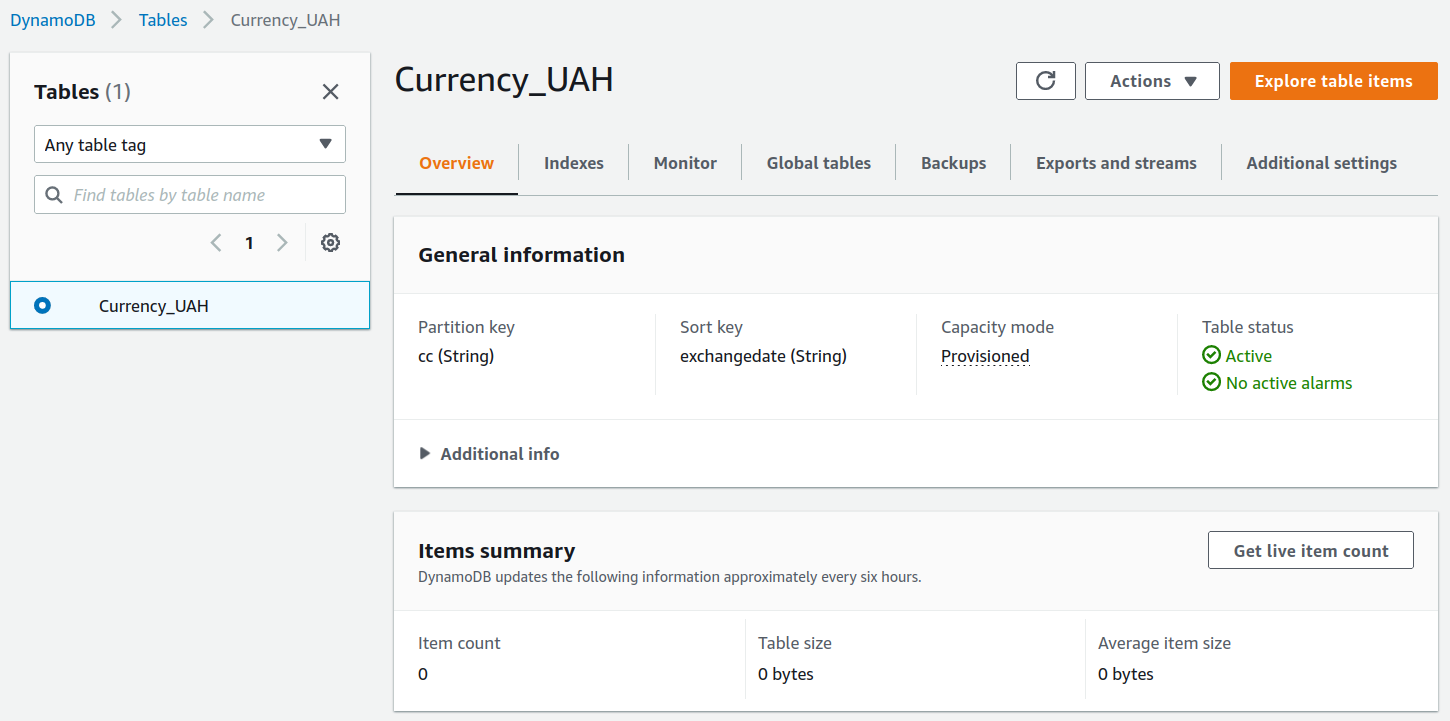
\includegraphics[width=0.85\linewidth]{1/1.2.png}}
    \caption{Інструменти новоствореної таблиці}
    \label{fig:explore table items AWS MC}
\end{figure}

\begin{figure}[H]
    \center{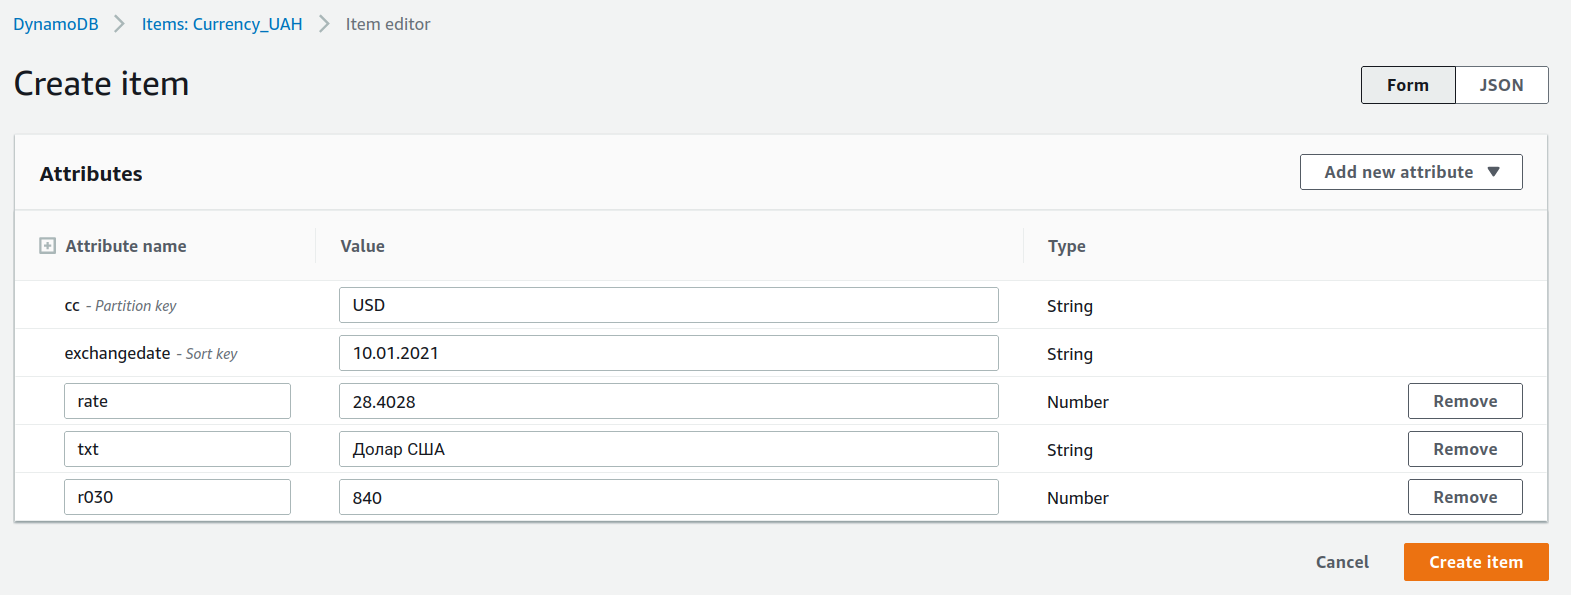
\includegraphics[width=0.85\linewidth]{1/1.4.png}}
    \caption{Додавання рядка до таблиці}
    \label{fig:add an item AWS MC}
\end{figure}

\begin{figure}[H]
    \center{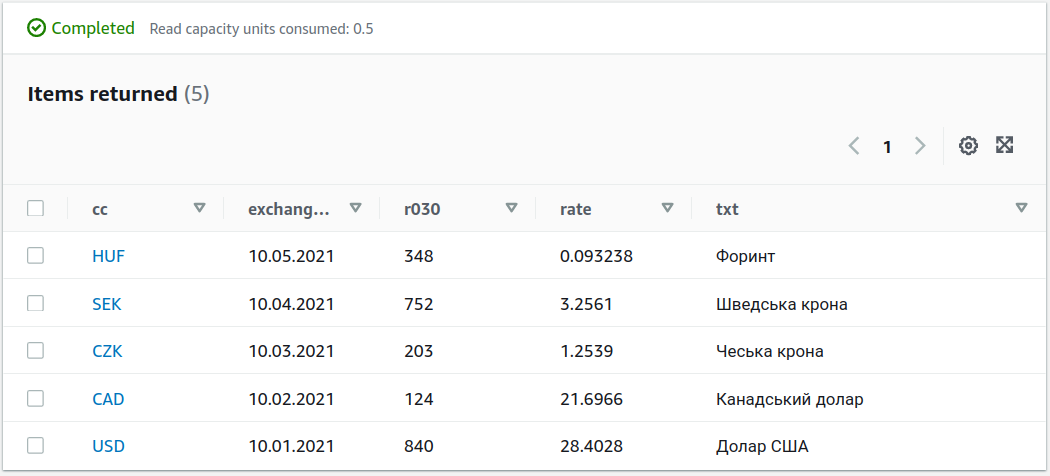
\includegraphics[width=0.85\linewidth]{1/1.6.png}}
    \caption{Наповнена даними таблиця}
    \label{fig:creation finished AWS MC}
\end{figure}

\subsubsection*{Пошук елементів таблиці}

Зайшовши у вкладку <<Explore table items>> в категорію <<Scan/Query items>> мож\-на здійснити пошук елементів 
в таблиці. Послідовно виконаємо три запити, які зоб\-ражено на Рис. \ref{fig:first scan AWS MC}-\ref{fig:third scan AWS MC}.

\begin{figure}[H]
    \begin{minipage}[H]{1\linewidth}
        \center{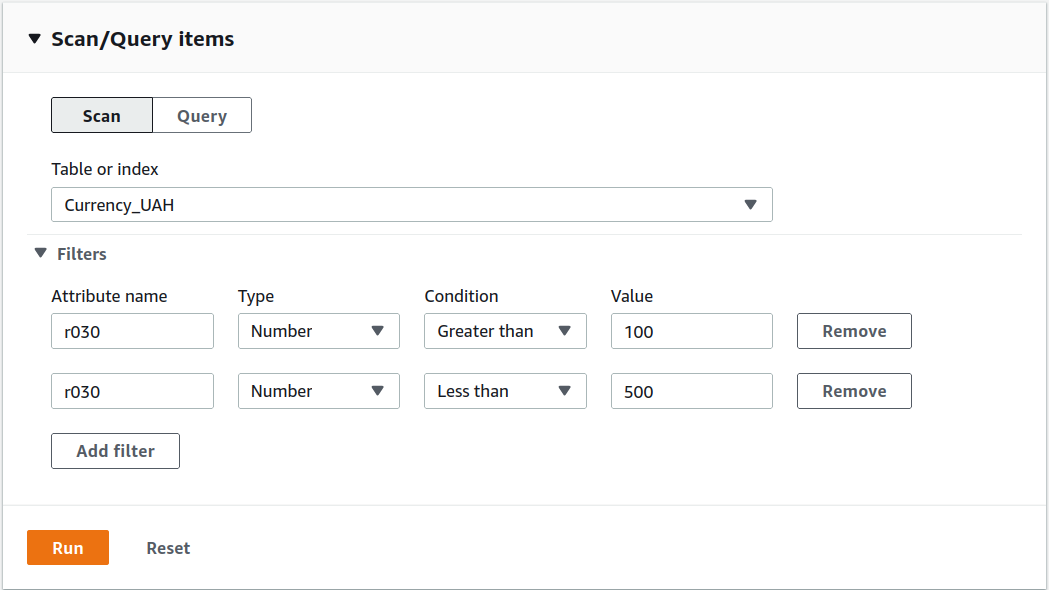
\includegraphics[width=0.8\linewidth]{1/2.1.png}}
    \end{minipage}
    \vfill
    \begin{minipage}[H]{1\linewidth}
        \vspace{0.5cm}\center{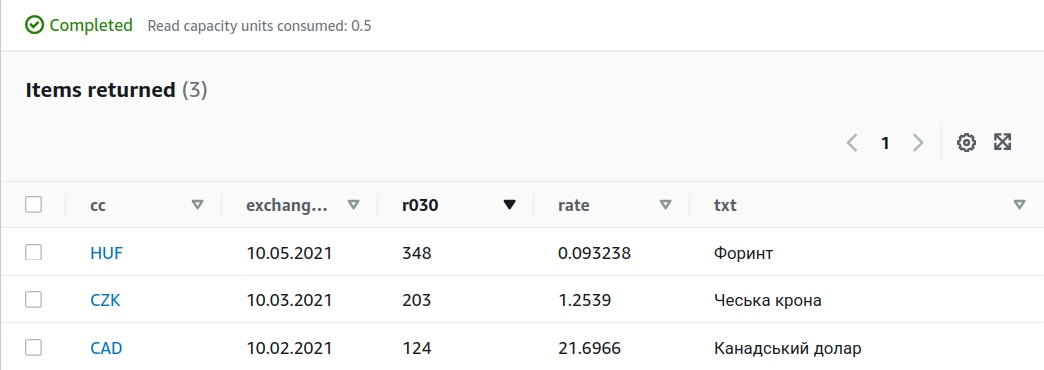
\includegraphics[width=0.8\linewidth]{1/2.2.png}}
        \caption{Перший запит}
        \label{fig:first scan AWS MC}
    \end{minipage}
\end{figure}

\begin{figure}[H]
    \center{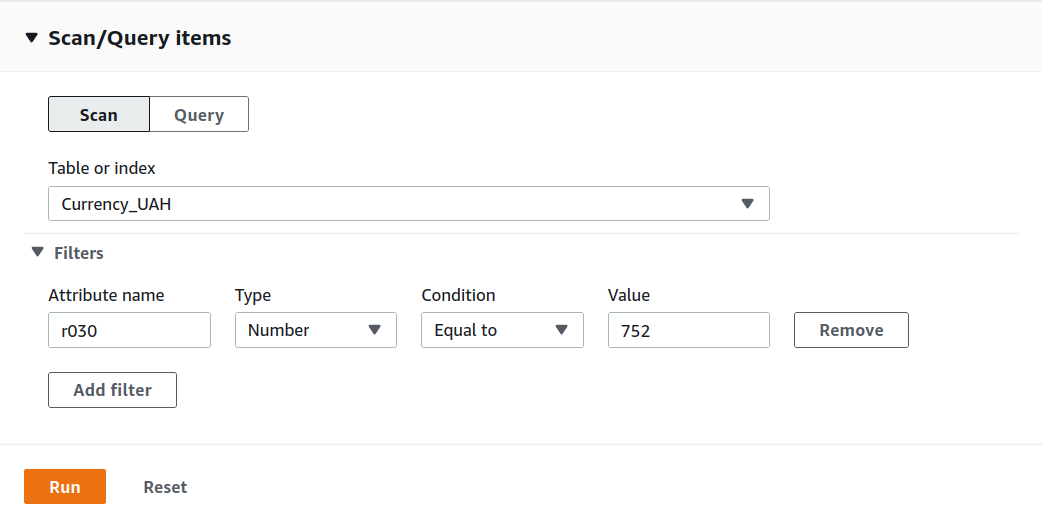
\includegraphics[width=0.8\linewidth]{1/2.3.png}}
\end{figure}

\begin{figure}[H]
    \center{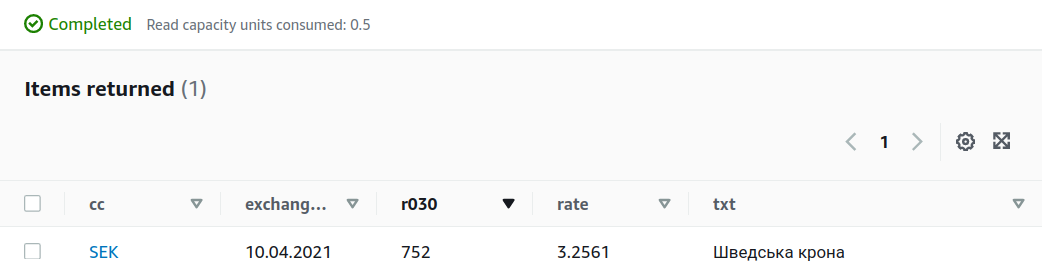
\includegraphics[width=0.8\linewidth]{1/2.4.png}}
    \caption{Другий запит}
    \label{fig:second scan AWS MC}
\end{figure}

\begin{figure}[H]
    \begin{minipage}[H]{1\linewidth}
        \center{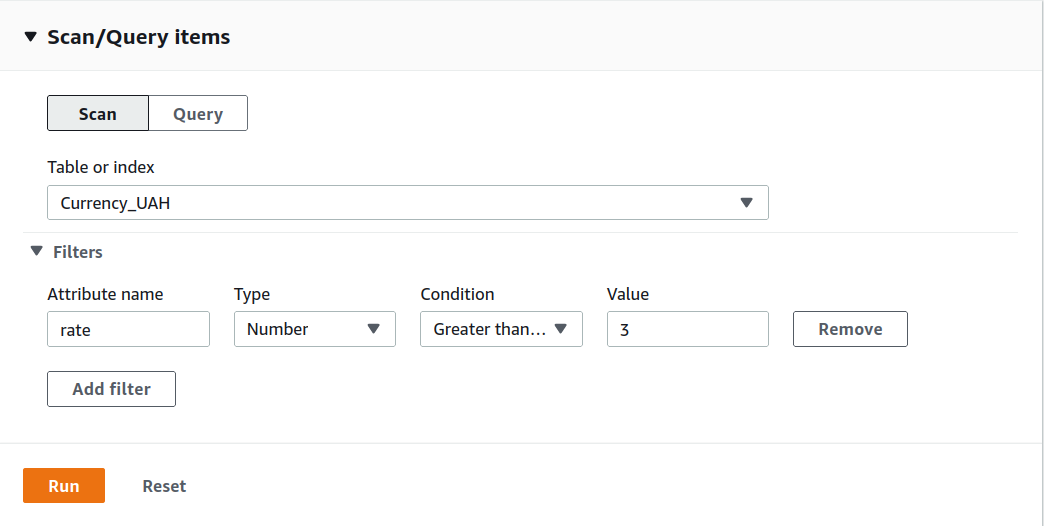
\includegraphics[width=0.8\linewidth]{1/2.5.png}}
    \end{minipage}
    \vfill
    \begin{minipage}[H]{1\linewidth}
        \vspace{0.1cm}\center{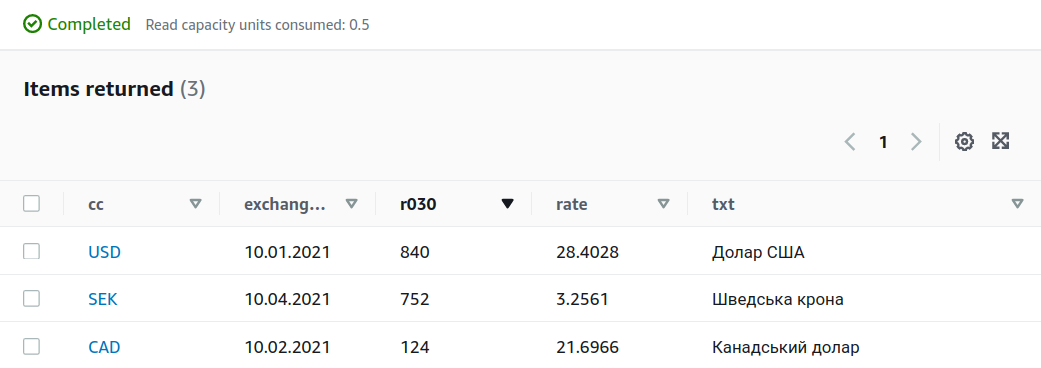
\includegraphics[width=0.8\linewidth]{1/2.6.png}}
        \caption{Третій запит}
        \label{fig:third scan AWS MC}
    \end{minipage}
\end{figure}

\subsubsection*{Видалення рядків таблиці}

Видалення рядків можна легко виконати, зробивши декілька кроків. Перш за все слід бути у розділі 
<<Explore table items>>. Навпроти рядка, який бажаємо видалити, слід поставити відмітку. Далі обираємо 
категорію <<Actions>>, де шукаємо варіант <<Delete items>>. Остаточно підтверджуємо операцію. Усі кроки 
показано на Рис. \ref{fig:delete the element AWS MC}.

\begin{figure}[H]
    \begin{minipage}[H]{1\linewidth}
        \center{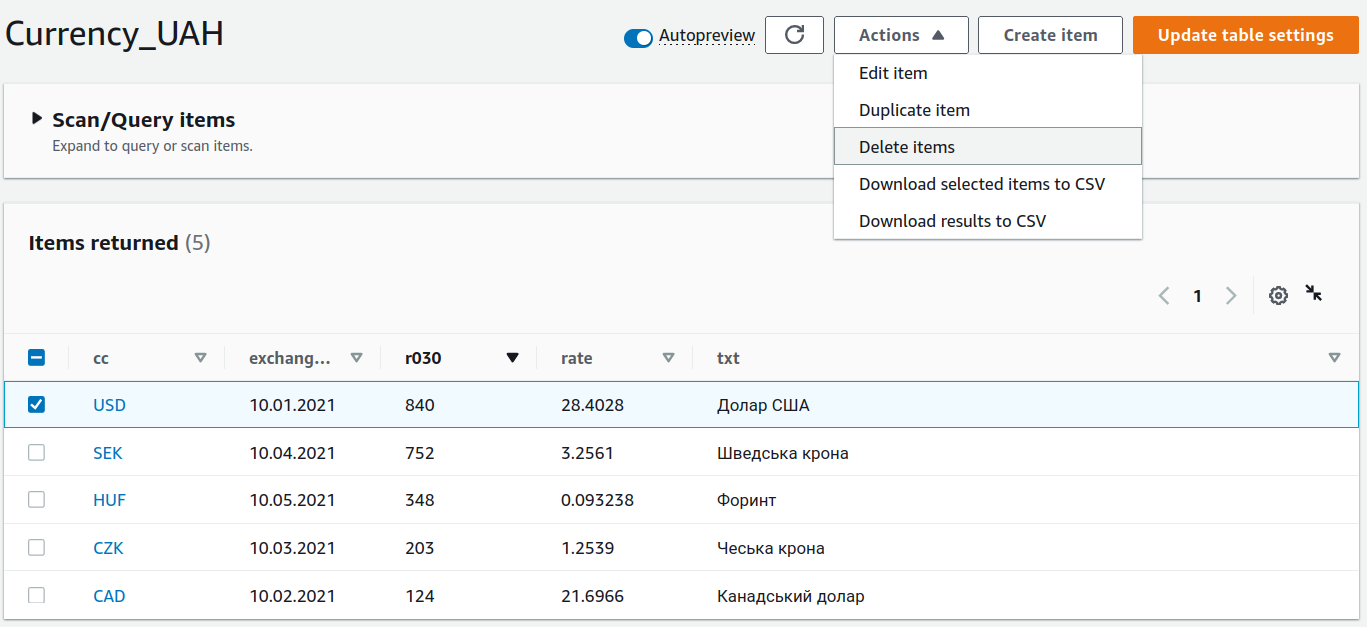
\includegraphics[width=0.8\linewidth]{1/3.1.png}}
    \end{minipage}
    \vfill
    \begin{minipage}[H]{1\linewidth}
        \vspace{0.5cm}\center{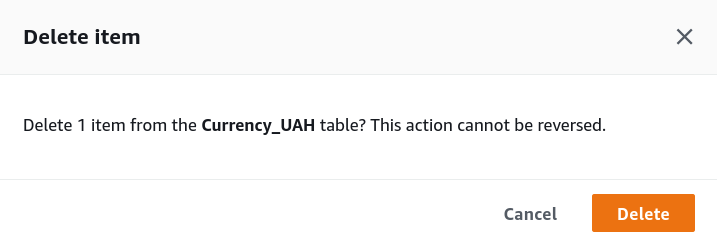
\includegraphics[width=0.8\linewidth]{1/3.2.png}}
        \caption{Видалення елементу з таблиці}
        \label{fig:delete the element AWS MC}
    \end{minipage}
\end{figure}

\subsection*{2. Робота з таблицею заcобами AWS CLI}

\subsubsection*{Створення таблиці}

Створимо ще одну таблицю, проте цього разу скористаємося засобами AWS Command Line Interface (AWS CLI). Для 
цього спершу підлючимося з консолі до інстансу (як це робилося у Лабораторній роботі \textnumero1). Надалі 
введемо таку команду: 

% [language=bash] https://tex.stackexchange.com/questions/84185/displaying-linux-commands-in-latex
\begin{lstlisting}[language=bash]
    aws dynamodb create-table \
    --table-name Currency_UAH_aws \
    --attribute-definitions \
        AttributeName=cc,AttributeType=S \
        AttributeName=exchangedate,AttributeType=S \
    --key-schema \
        AttributeName=cc,KeyType=HASH \
        AttributeName=exchangedate,KeyType=RANGE \
    --provisioned-throughput \
        ReadCapacityUnits=10,WriteCapacityUnits=5
\end{lstlisting}

Рядком 2 оголосимо ім'я таблиці, рядками 3-5, 6-8 створимо дві колонки й оголосимо їх складеним Primary key 
(складові HASH та RANGE відповідно). Останнім атрибутом \texttt{{-}{-}provisioned-throughput} вказуємо кількість 
зчитувань/записів за секунду для нашої таблиці. Детальніше про параметри цього атрибуту за 
\href{https://docs.aws.amazon.com/amazondynamodb/latest/developerguide/ProvisionedThroughput.html#ProvisionedThroughput.CapacityUnits.Read}{посиланням}.

\begin{figure}[H]
    \begin{minipage}[H]{1\linewidth}
        \center{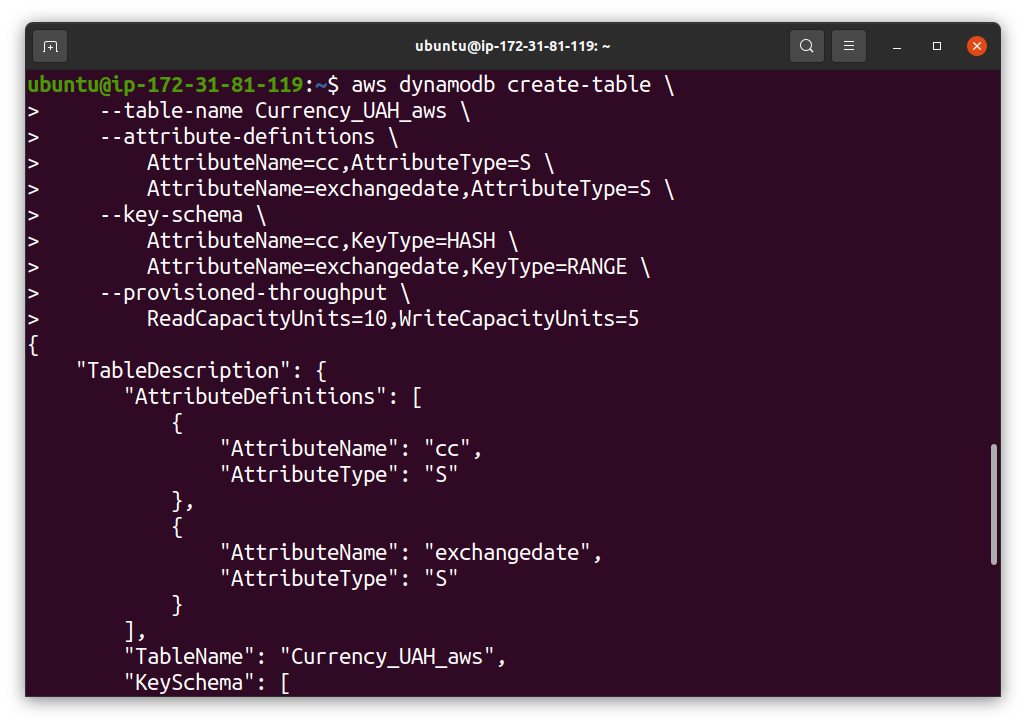
\includegraphics[width=1\linewidth]{2/1.1.png}}
    \end{minipage}
    \vfill
    \begin{minipage}[H]{1\linewidth}
        \center{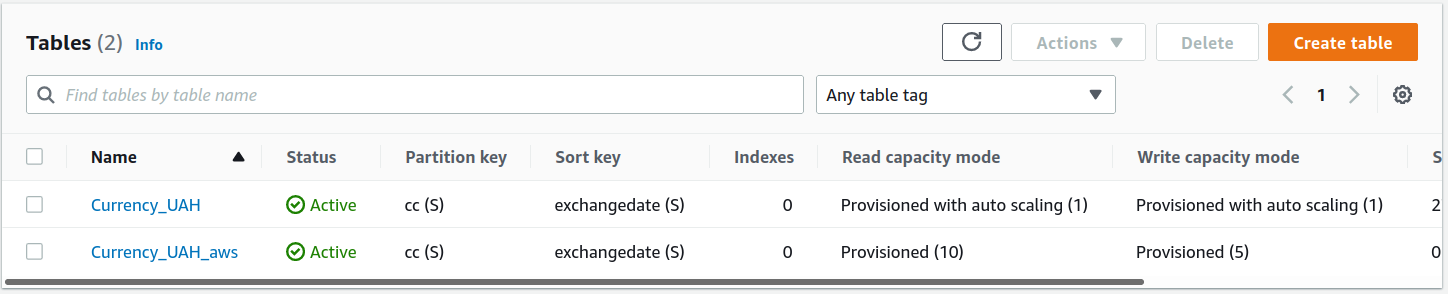
\includegraphics[width=1\linewidth]{2/1.2.png}}
        \caption{Створення таблиці засобами AWS CLI}
        \label{fig:create table AWS CLI}
    \end{minipage}
\end{figure}

\subsubsection*{Додавання рядків до таблиці}

Поступово додамо 4 рядки до новоствореної таблиці <<Currency\_UAH\_aws>>. Зауважимо, що інформація про 
рядок має бути подана у json-форматі. Тож виконаємо команду виду

\begin{lstlisting}[language=bash, stringstyle=\small\ttfamily, emphstyle={[1]\small\ttfamily}]
    aws dynamodb put-item \
    --table-name Currency_UAH_aws  \
    --item \
        '{"r030": {"N": "124"}, "txt": {"S": "Канадський долар"}, "rate": {"N": "21.6966"}, "cc": {"S": "CAD"}, "exchangedate": {"S": "10.02.2021"}}' \
   --return-consumed-capacity TOTAL
\end{lstlisting}

На Рис. \ref{fig:add first item AWS CLI} та Рис. \ref{fig:add second item AWS CLI} виконано додавання двох елементів. 
Фінальний вигляд таблиця отримає на Рис. \ref{fig:creation finished AWS CLI}.

\begin{figure}[H]
    \begin{minipage}[H]{1\linewidth}
        \center{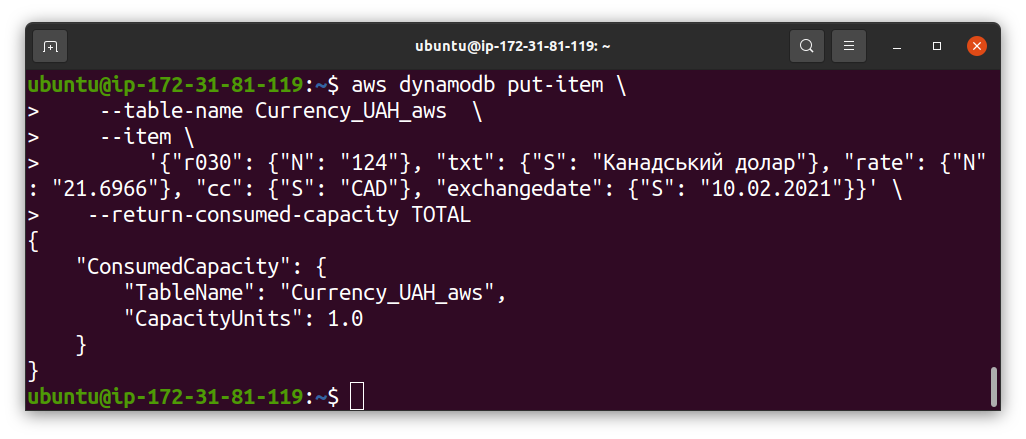
\includegraphics[width=0.9\linewidth]{2/2.1.png}}
    \end{minipage}
    \vfill
    \begin{minipage}[H]{1\linewidth}
        \center{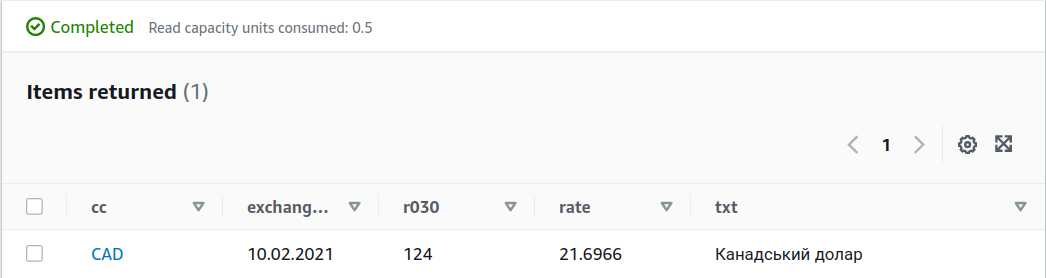
\includegraphics[width=0.9\linewidth]{2/2.2.png}}
        \caption{Додавання першого рядка до таблиці}
        \label{fig:add first item AWS CLI}
    \end{minipage}
\end{figure}

\begin{figure}[H]
    \begin{minipage}[H]{1\linewidth}
        \center{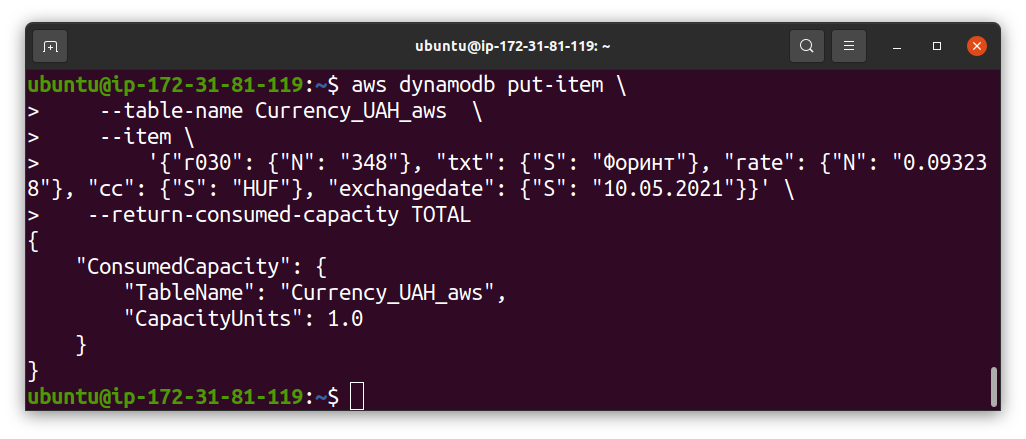
\includegraphics[width=0.9\linewidth]{2/2.3.png}}
    \end{minipage}
    \vfill
    \begin{minipage}[H]{1\linewidth}
        \center{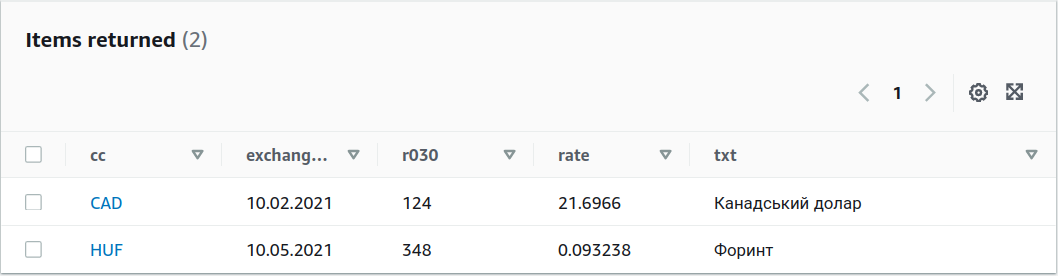
\includegraphics[width=0.9\linewidth]{2/2.4.png}}
        \caption{Додавання другого рядка до таблиці}
        \label{fig:add second item AWS CLI}
    \end{minipage}
\end{figure}

\begin{figure}[H]
    \center{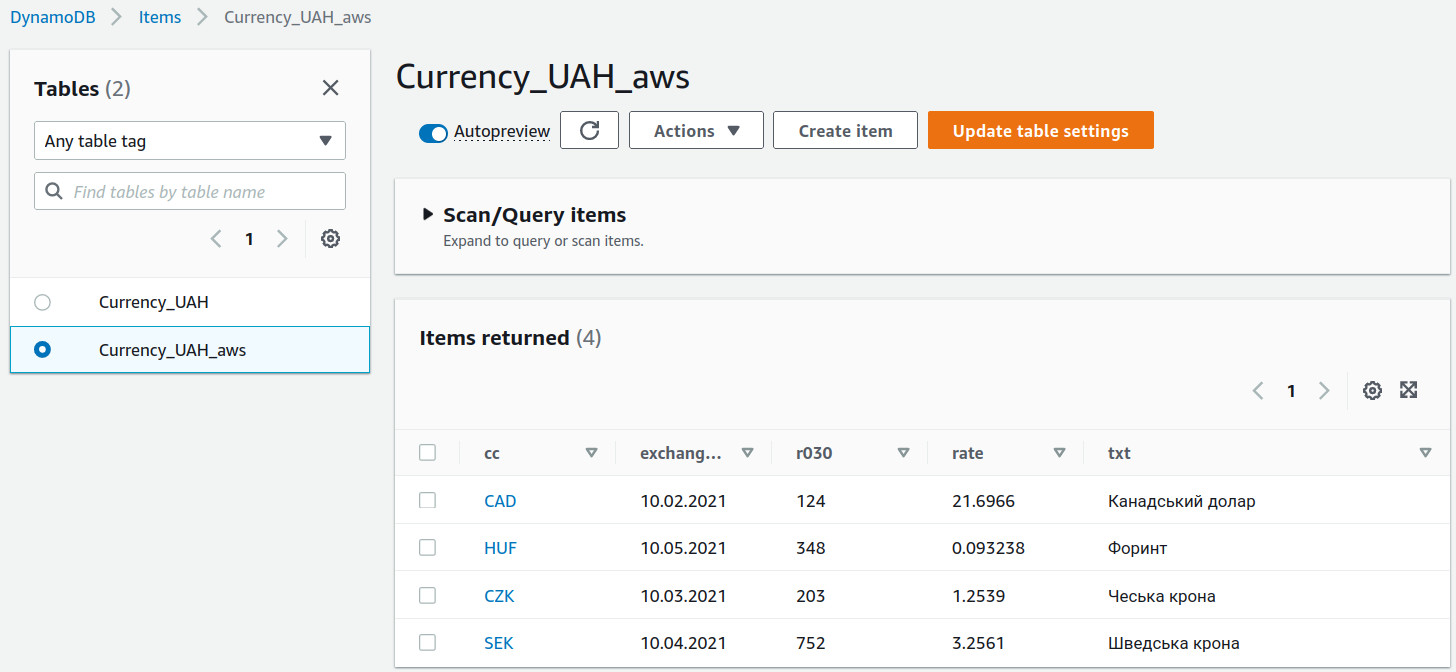
\includegraphics[width=1\linewidth]{2/2.9.png}}
    \caption{Наповнена даними таблиця}
    \label{fig:creation finished AWS CLI}
\end{figure}

\subsubsection*{Пошук елементів таблиці}

Для пошуку певних рядків виконаємо команду, яка зображена на Рис. \ref{fig:first query AWS CLI}.

\begin{figure}[H]
    \center{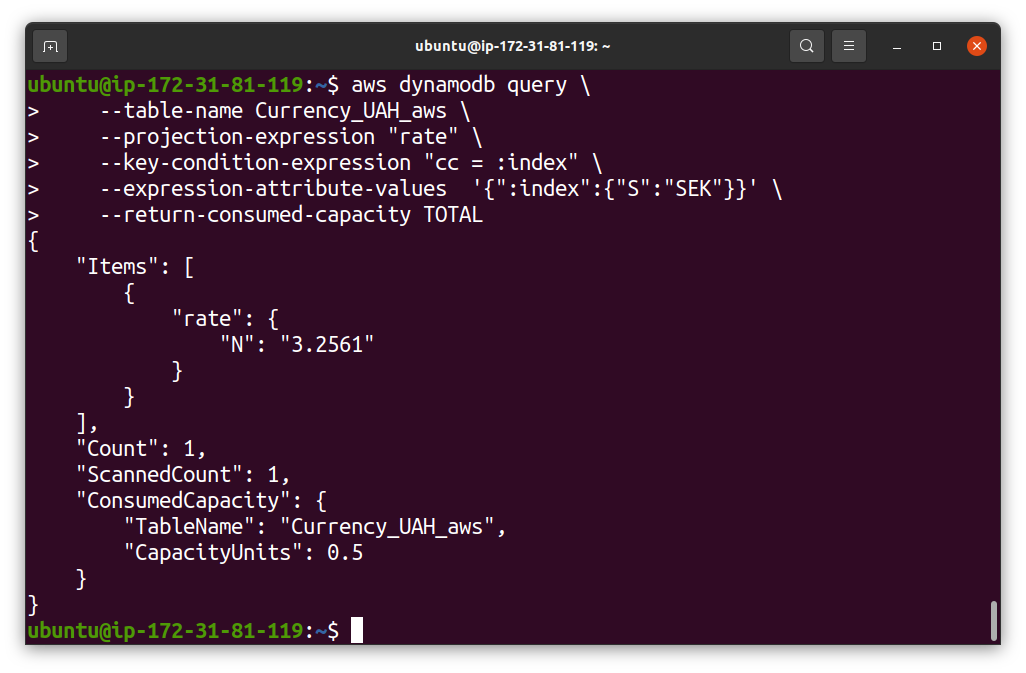
\includegraphics[width=1\linewidth]{2/3.1.png}}
    \caption{Перший запит}
    \label{fig:first query AWS CLI}
\end{figure}

\newpage

Як бачимо, команда має вид

\begin{lstlisting}[language=bash, stringstyle=\small\ttfamily, emphstyle={[1]\small\ttfamily}]
    aws dynamodb query \
    --table-name Currency_UAH_aws \
    --projection-expression "rate" \
    --key-condition-expression "cc = :index" \
    --expression-attribute-values  '{":index":{"S":"SEK"}}' \
    --return-consumed-capacity TOTAL
\end{lstlisting}

У рядках 4-5 через проміжний параметр \texttt{index} вказують рівність шуканої валюти: \texttt{"cc"$=$"SEK"}, 
а у рядку номер 3 ми додатково вказуємо, що нас цікавить виключ\-но значення \texttt{"rate"} обраної валюти 
(на противгу запиту на Рис. \ref{fig:second query AWS CLI}, де на вихід отримуємо весь рядок з шуканою валютою).

\begin{figure}[H]
    \center{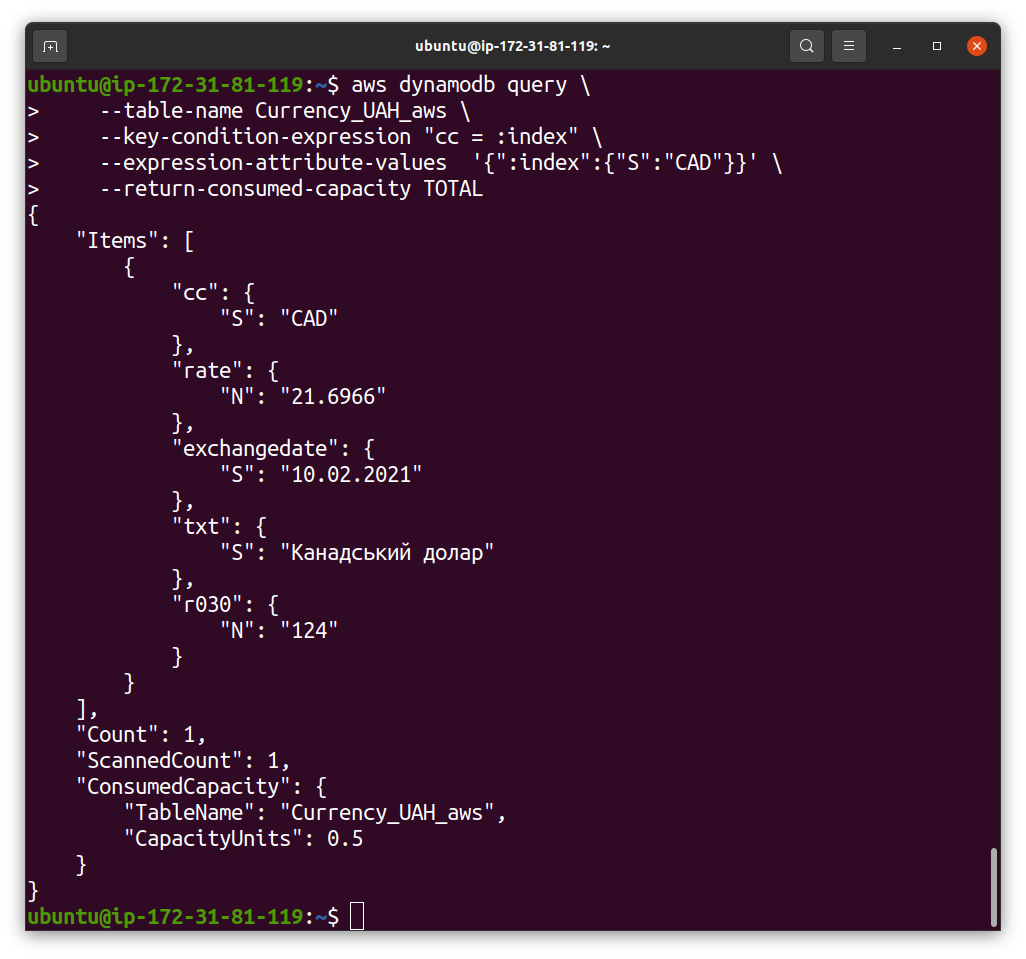
\includegraphics[width=1\linewidth]{2/3.2.png}}
    \caption{Другий запит}
    \label{fig:second query AWS CLI}
\end{figure}

\subsubsection*{Видалення рядків таблиці}

Команда видалення рядка має просту структуру: необхідно лише вказати повне значення складеного Primary key. 

\begin{lstlisting}[language=bash, stringstyle=\small\ttfamily, emphstyle={[1]\small\ttfamily}]
    aws dynamodb delete-item \
    --table-name Currency_UAH_aws \
    --key '{"cc": {"S": "CZK"},"exchangedate": {"S": "10.03.2021"}}' \
    --return-values ALL_OLD \
    --return-consumed-capacity TOTAL \
    --return-item-collection-metrics SIZE
\end{lstlisting}

Порівнявши таблиці на Рис. \ref{fig:creation finished AWS CLI} та Рис. \ref{fig:delete the element AWS CLI} 
переконуємося, що видалення успішне.

\begin{figure}[H]
    \begin{minipage}[H]{1\linewidth}
        \center{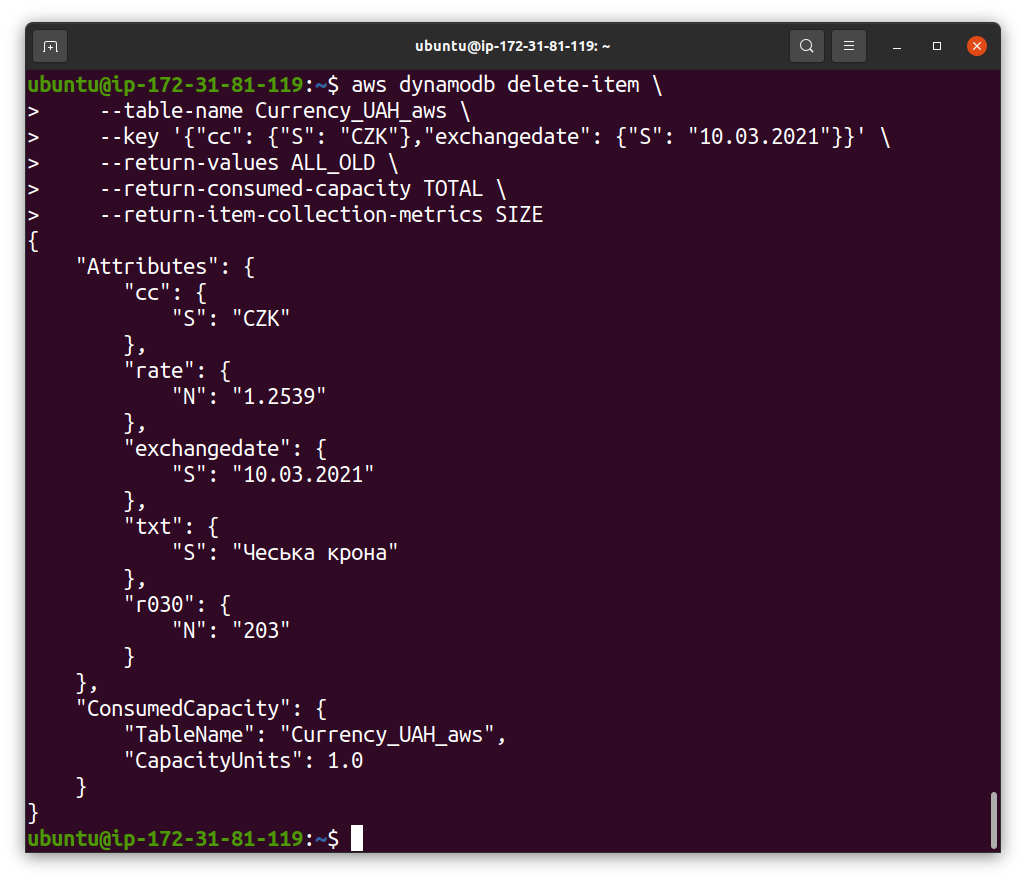
\includegraphics[width=0.85\linewidth]{2/4.1.png}}
    \end{minipage}
    \vfill
    \begin{minipage}[H]{1\linewidth}
        \center{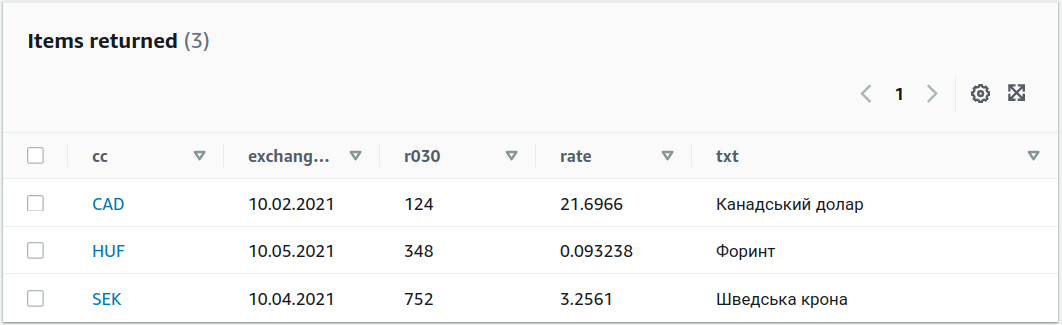
\includegraphics[width=0.85\linewidth]{2/4.2.png}}
        \caption{Видалення рядка з таблиці}
        \label{fig:delete the element AWS CLI}
    \end{minipage}
\end{figure}

\subsection*{3. Робота з таблицею через додаток NoSQL Workbench}

\subsubsection*{Створення таблиці}

Перш за все слід встановити додаток NoSQL Workbench для необхідної операційної системи, перейшовши за
\href{https://docs.aws.amazon.com/amazondynamodb/latest/developerguide/workbench.settingup.html}{посиланням}. 
Конкретні кроки, які слід виконати після завантаження файлу на Linux, описані на цьому 
\href{https://itsfoss.com/use-appimage-linux/}{сайті}. В цілому, робота з файлом розширення .AppImage не викликала 
труднощів. Тож здійснюємо вхід у додаток й опиняємося на головні сторінці (Рис. \ref{fig:main page NoSQL}).

\begin{figure}[H]
    \center{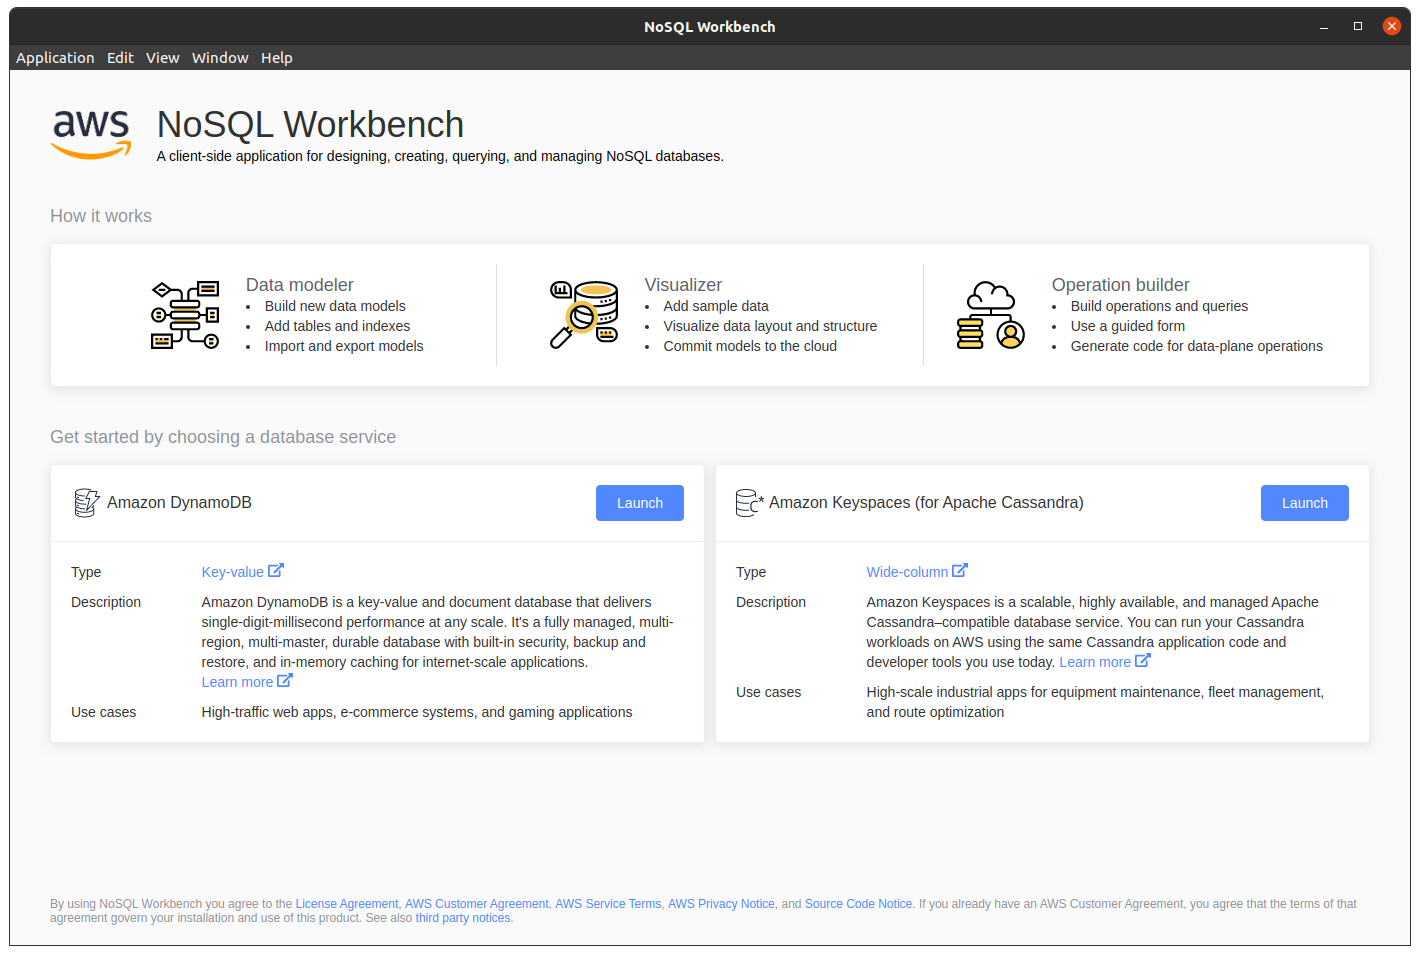
\includegraphics[width=1\linewidth]{3/1.1.png}}
    \caption{Головна сторінка додатку NoSQL Workbench}
    \label{fig:main page NoSQL}
\end{figure}

\begin{figure}[H]
    \begin{minipage}[H]{0.44\linewidth}
        \center{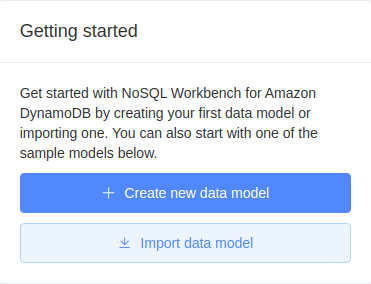
\includegraphics[width=0.8\linewidth]{3/1.2.png}}
    \end{minipage}
    \hfill
    \begin{minipage}[H]{0.54\linewidth}
        \center{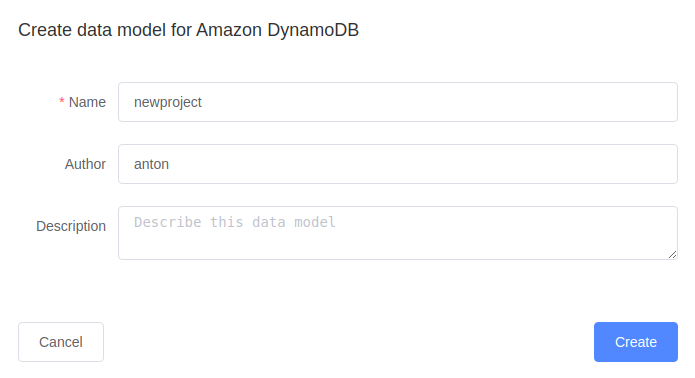
\includegraphics[width=1\linewidth]{3/1.3.png}}
    \end{minipage}
    \caption{Створення нової моделі даних}
    \label{fig:create a model NoSQL}
\end{figure}

Отже, обираємо <<Launch>> для Amazon DynamoDB (Рис. \ref{fig:main page NoSQL}). Далі створюємо так звану 
нову модель даних (Рис.~\ref{fig:create a model NoSQL}). Тож у новоствореній моделі вже маємо можливість 
створити таблицю із потрібною нам назвою та потрібними для нас колонками. Процес створення та отриманий 
результат показаний на Рис. 
\ref{fig:create a table NoSQL}. 

\begin{figure}[H]
    \begin{minipage}[H]{0.49\linewidth}
        \center{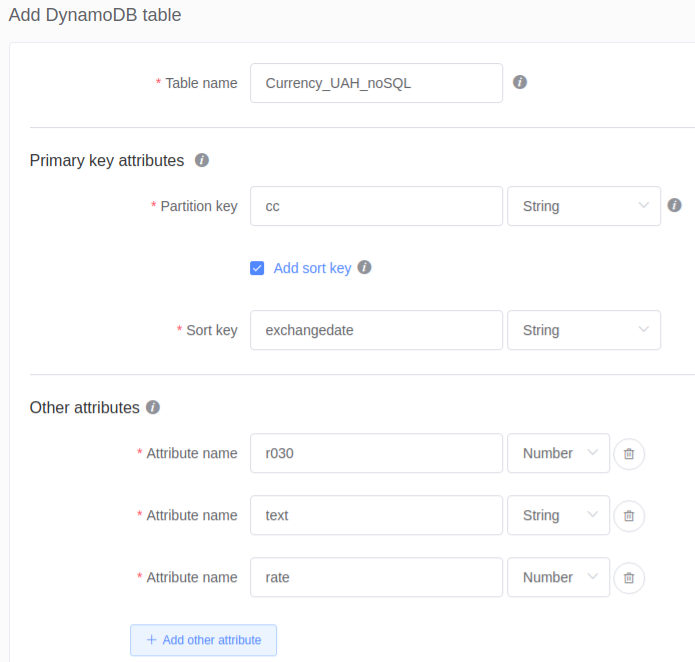
\includegraphics[width=0.9\linewidth]{3/1.4.png}}
    \end{minipage}
    \hfill
    \begin{minipage}[H]{0.49\linewidth}
        \center{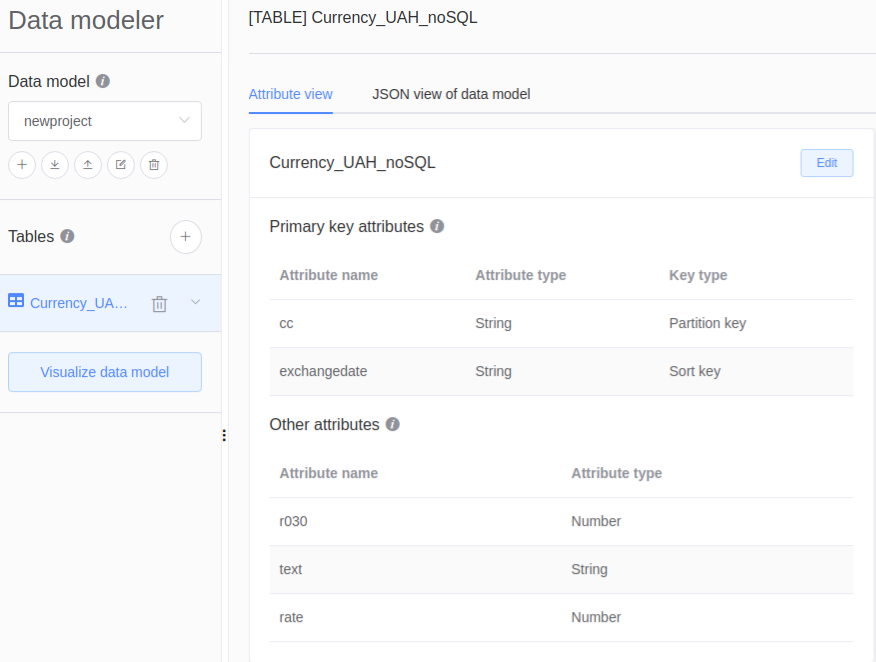
\includegraphics[width=1\linewidth]{3/1.5.png}}
    \end{minipage}
    \caption{Створення таблиці даних}
    \label{fig:create a table NoSQL}
\end{figure}

\subsubsection*{Підключення таблиці до існуючого DynamoDB}

Здійснимо підключення створеної таблиці до DynamoDB на акаунті Amazon. Оберемо розділ <<Visualizer>> та введемо 
усі необхідні параметри користувача сервісу Amazon (Рис. \ref{fig:commint NoSQL}). Переконаємося в успішності 
підключення (Рис. \ref{fig:commint succeed NoSQL}).

\begin{figure}[H]
    \center{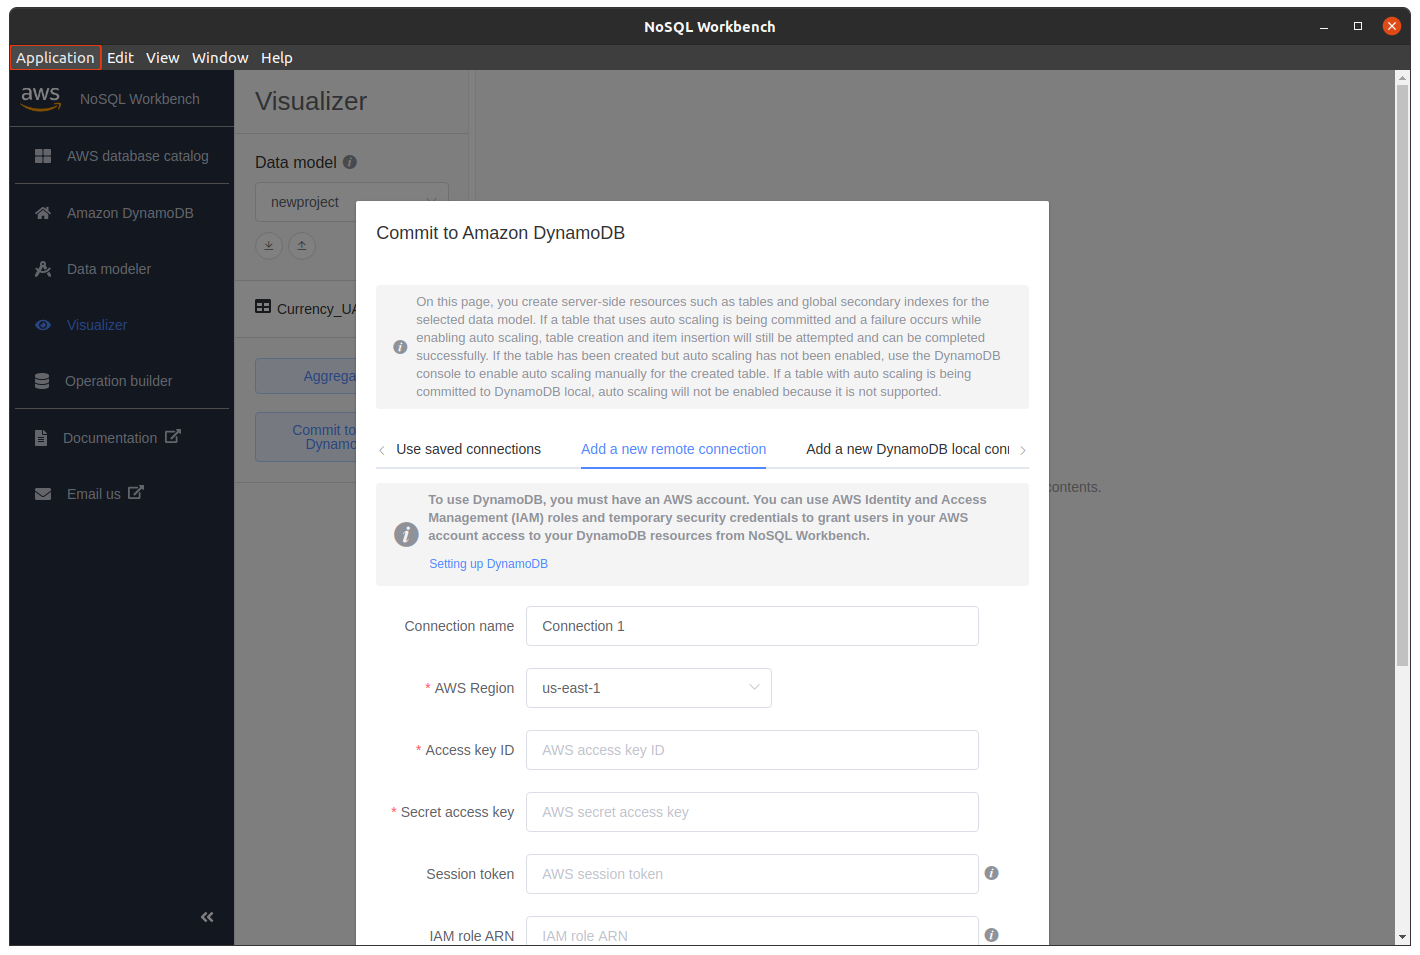
\includegraphics[width=0.8\linewidth]{3/2.1.png}}
    \caption{Підключення таблиці до DynamoDB}
    \label{fig:commint NoSQL}
\end{figure}

\begin{figure}[H]
    \center{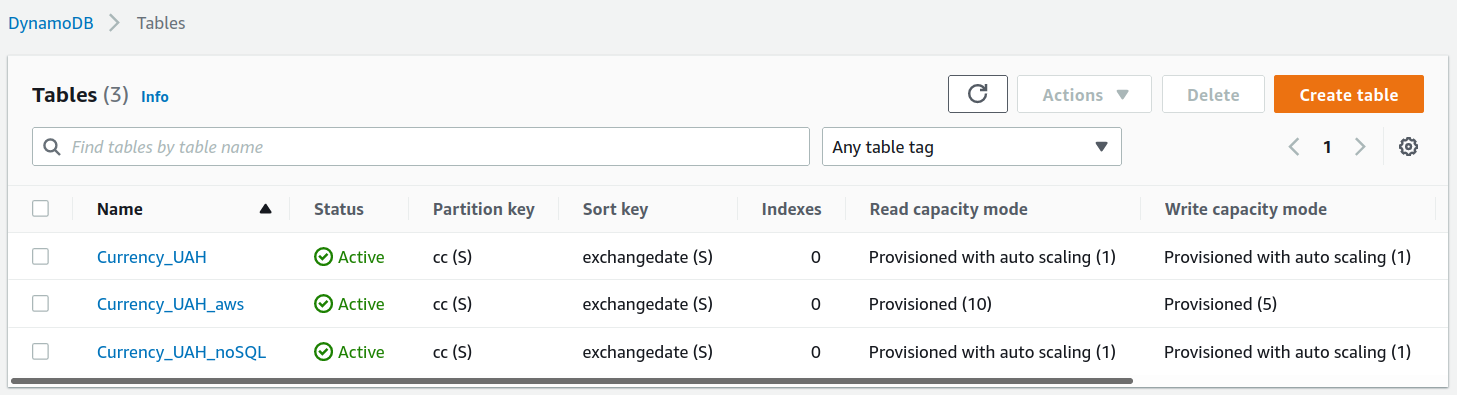
\includegraphics[width=1\linewidth]{3/2.3.png}}
    \caption{Таблиця <<Currency\_UAH\_noSQL>> успішно підключена}
    \label{fig:commint succeed NoSQL}
\end{figure}

\subsection*{4. Робота з таблицею засобами Python (додаткове завдання)}

\subsubsection*{Створення таблиці}

Перш за все запустимо вже встановлений у Лабораторній роботі \textnumero2 jupyter notebook на інстансі та 
працюватимемо з ним з локального робочого місця. Пiдключимося з консолi до iнстансу й знову виконаємо команди:
\begin{align*}
    &\texttt{jupyter notebook {-}{-}no-browser {-}{-}port 8889} && \text{на інстансі} \\
    &\texttt{ssh -i lab.pem -N -f -L localhost:8888:localhost:8889} && \text{локально}
\end{align*}

Створивши файл (наприклад, з на звою \texttt{Lab2.ipynb}), напишемо рядки коду, які зображено на Лістингу 
\ref{create a table}. Придивившись, легко впізнаємо абсолютно аналогічну схему команд, як це було у випадку 
роботи з таблицями засобами AWS CLI (Рис.~\ref{fig:create table AWS CLI}).

\lstinputlisting[firstnumber=1, firstline=1, lastline=31, label = create a table, caption = Створення таблиці]{Code/DynamoDB_part1.py}

\begin{figure}[H]
    \center{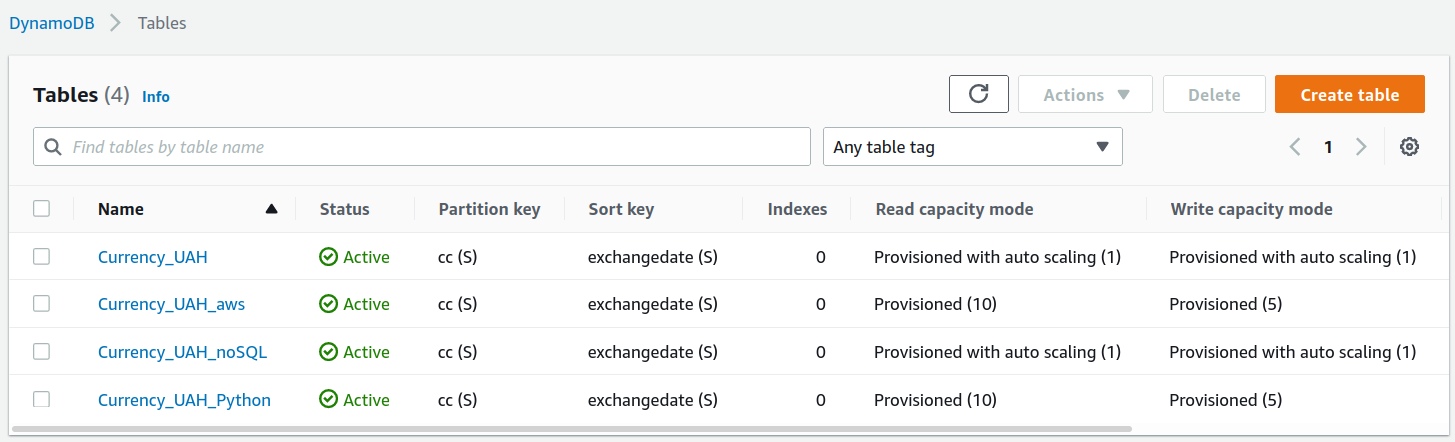
\includegraphics[width=1\linewidth]{4/1.png}}
    \caption{Таблиця <<Currency\_UAH\_Python>> успішно створена}
    \label{fig:table Python}
\end{figure}

\subsubsection*{Додавання рядків до таблиці}

Послідовно додамо 4 рядки, виконуючи відповідну команду (Лістинг \ref{add an item}). Таким чином отримаємо 
заповнену даними й остаточно сформовану таблицю (Рис. \ref{fig:full table Python}).

\lstinputlisting[firstnumber=33, firstline=33, lastline=52, label = add an item, caption = Додавання двох рядків]{Code/DynamoDB_part1.py}

\begin{figure}[H]
    \center{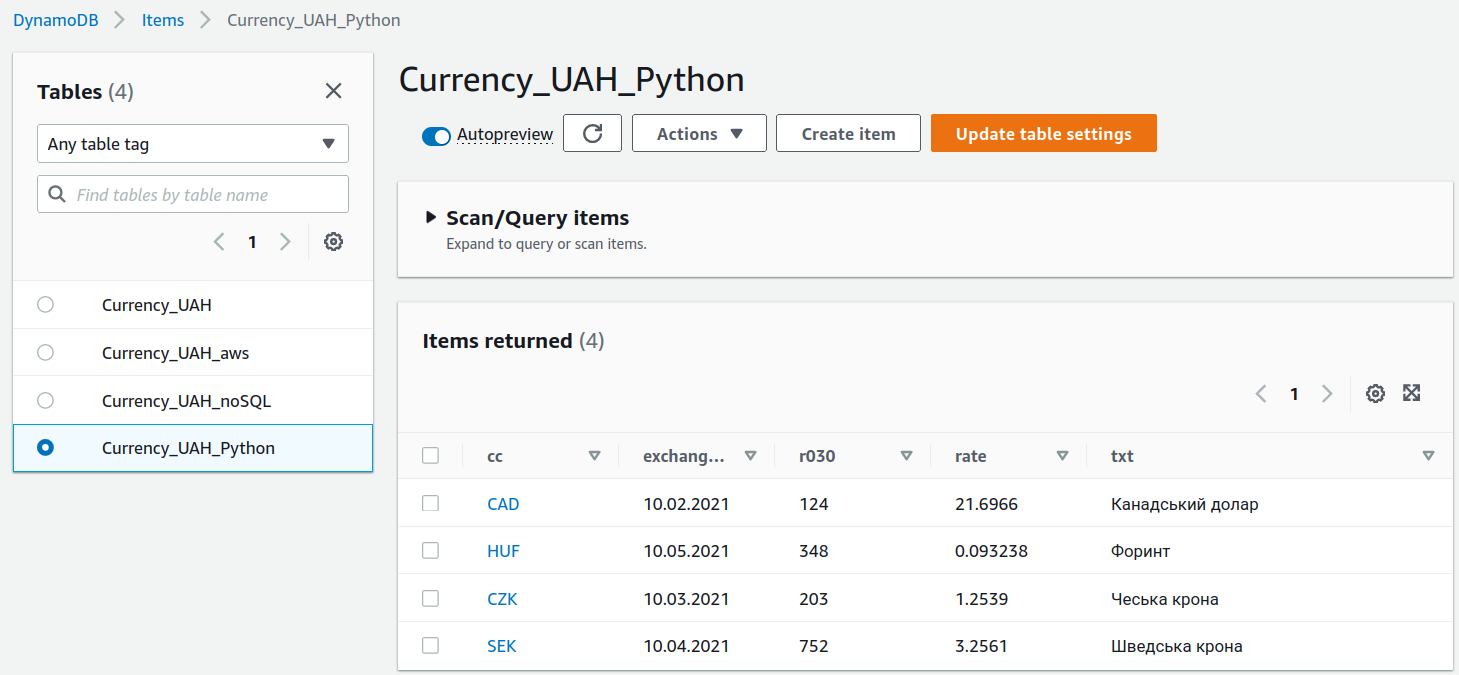
\includegraphics[width=1\linewidth]{4/2.png}}
    \caption{Наповнена даними таблиця}
    \label{fig:full table Python}
\end{figure}

\subsubsection*{Пошук елементів таблиці}

\lstinputlisting[firstnumber=72, firstline=1, lastline=12, label = find an item, caption = Виконання пошукових запитів]{Code/DynamoDB_part2.py}

\begin{figure}[H]
    \center{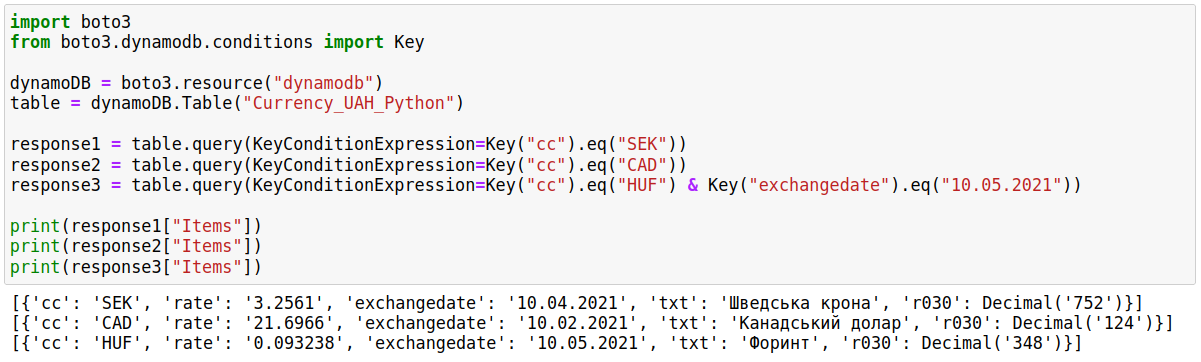
\includegraphics[width=1\linewidth]{4/3.png}}
    \caption{Результати запитів}
    \label{fig:Query Python}
\end{figure}

\subsubsection*{Видалення рядків таблиці}

Команда видалення рядка має просту структуру: необхідно лише вказати повне значення складеного Primary key 
(Лістинг \ref{delete an item}). 

\lstinputlisting[firstnumber=85, firstline=14, lastline=17, label = delete an item, caption = Видалення рядка]{Code/DynamoDB_part2.py}

Порівнявши таблиці на Рис. \ref{fig:full table Python} та Рис. \ref{fig:delete an item Python} переконуємося, 
що видалення рядка з таблиці пройшло успішно.

\begin{figure}[H]
    \center{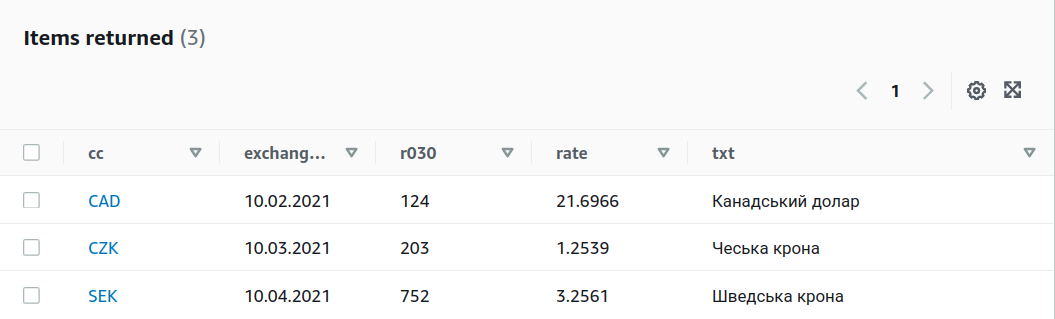
\includegraphics[width=1\linewidth]{4/4.png}}
    \caption{Рядок успішно видалений}
    \label{fig:delete an item Python}
\end{figure}

\end{document}